\section{Patryk Skowron}

Dodaję wyrażenie matematyczne w tekście
$1^n+ {2 \choose k}=\sum_{j=1}^{i} a_{ij}$
oraz pod tekstem:
\[\{\forall_{\alpha>0} \exists_{\gamma>0} : \alpha+\beta=\gamma\}\]

\begin{figure}[htbp]
    \centering
    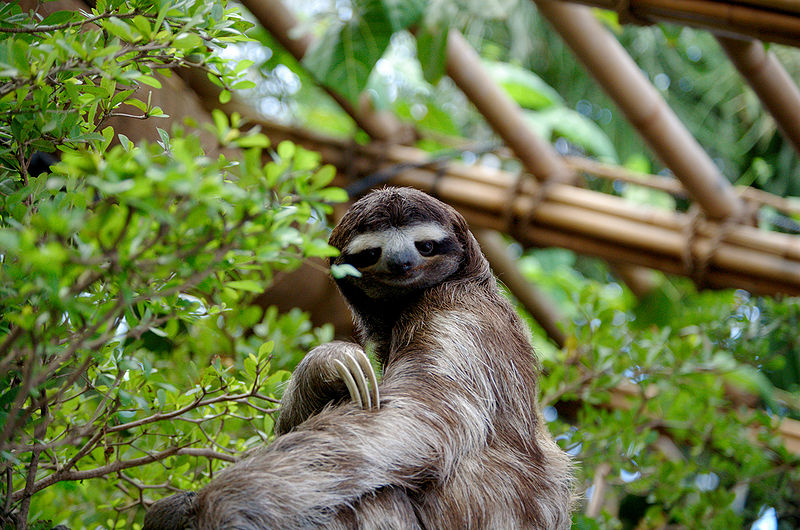
\includegraphics[scale=0.3]{pictures/leniwiec.jpg}
    \caption{Spokojny leniwiec}
    \label{fig:ln}
\end{figure}

Tabela:~\ref{tab:patr}
\begin{table}[htbp]
    \centering
\begin{tabular}{|c|c|c|c|l}
\cline{1-4}
\textbf{x\textbackslash{}y} & 1     & 2     & 3     &  \\ \cline{1-4}
1                           & (1,1) & (1,2) & (1,3) &  \\ \cline{1-4}
2                           & (2,1) & (2,2) & (2,3) &  \\ \cline{1-4}
3                           & (3,1) & (3,2) & (3,3) &  \\ \cline{1-4}
\end{tabular}
\caption{Współrzędne}
\label{tab:patr}
\end{table}

\newline

Lista numerowana:
\begin{enumerate}
    \item Przedmiot 1
    \item Przedmiot 2
    \item Przedmiot 3
\end{enumerate}

\newpage

Lista nienumerowana:
\begin{itemize}
    \item[+] It1
    \item[-] It2
    \item[!] It3
\end{itemize}

\textbf{Python} – język programowania \underline{wysokiego poziomu} ogólnego przeznaczenia, o rozbudowanym pakiecie bibliotek standardowych, którego ideą przewodnią jest \emph{czytelność i klarowność} kodu źródłowego. Jego składnia cechuje się przejrzystością i zwięzłością.

\textit{Python} wspiera różne \underline{paradygmaty} programowania: obiektowy, imperatywny oraz w mniejszym stopniu funkcyjny. Posiada w pełni dynamiczny system typów i automatyczne zarządzanie pamięcią, będąc w tym podobnym do języków \textit{Perl, Ruby, Scheme czy Tcl.} Podobnie jak inne języki dynamiczne jest często używany jako język skryptowy. Interpretery \emph{Pythona} są dostępne na wiele systemów operacyjnych.

Źródło: \emph{https://pl.wikipedia.org/wiki/Python}